\begin{section}{Resultados}

\subsection{Sa�da das Consultas}
\subsubsection{\textbf{Rela��o 1 Folha de Frequ�ncia}}

\begin{figure}[!h]
    \centering
    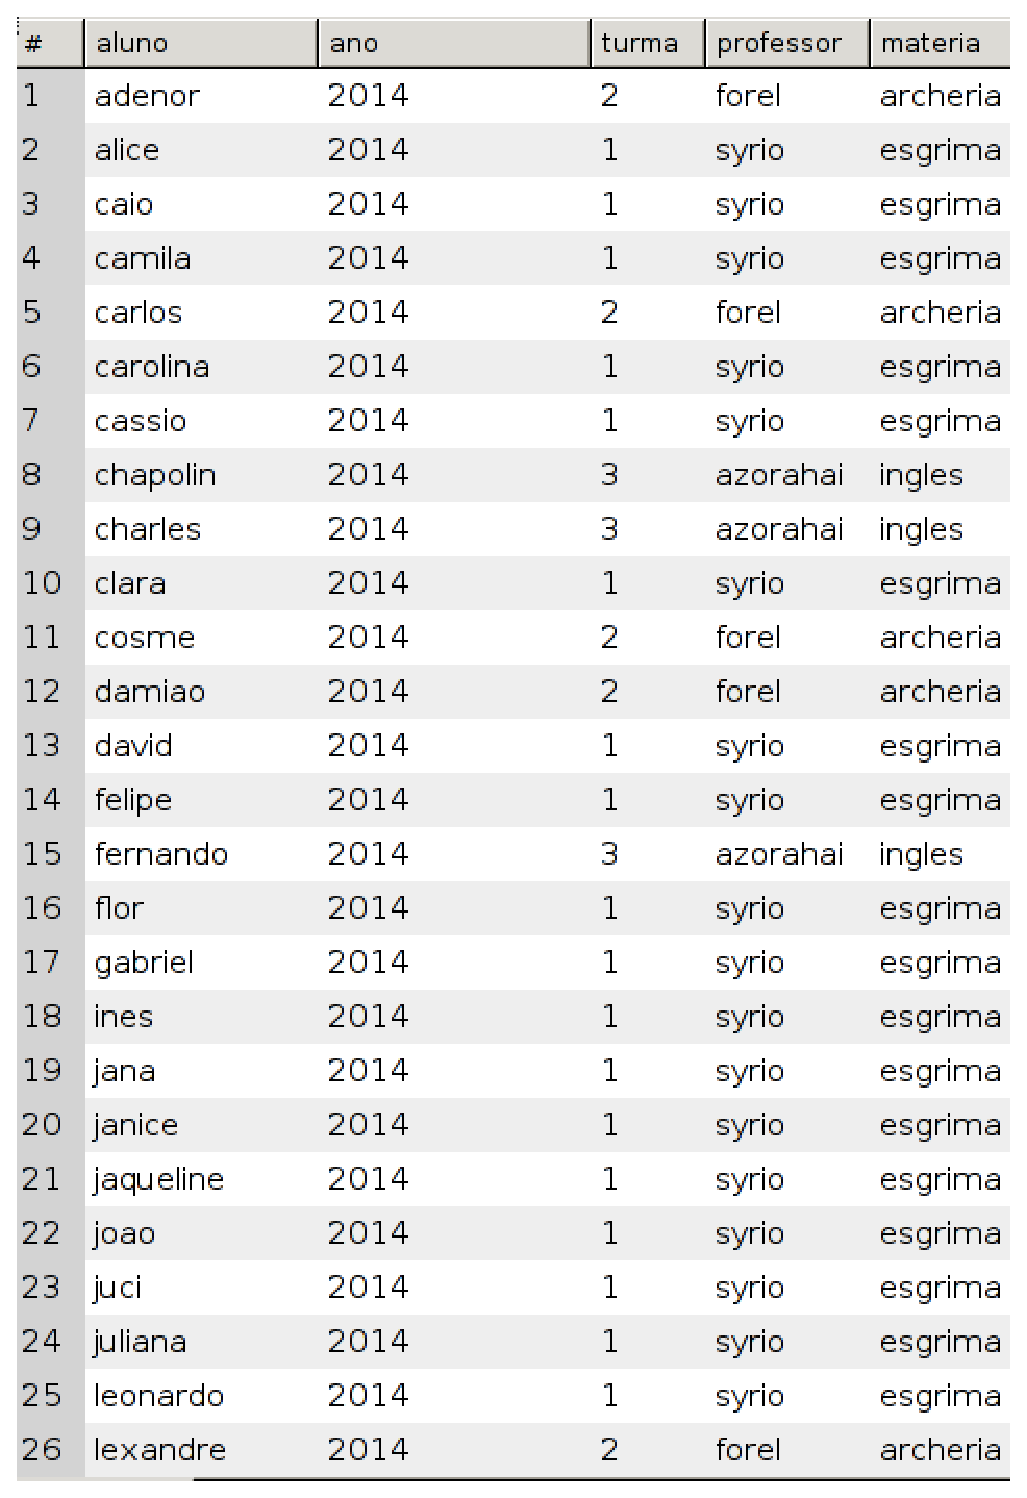
\includegraphics[width=.7\textwidth]{Figures/r11}
    \caption{Sa�da da Consulta 1 \textbf{parte 1}}
    \label{fig:r11}
\end{figure}

\begin{figure}[!h]
    \centering
    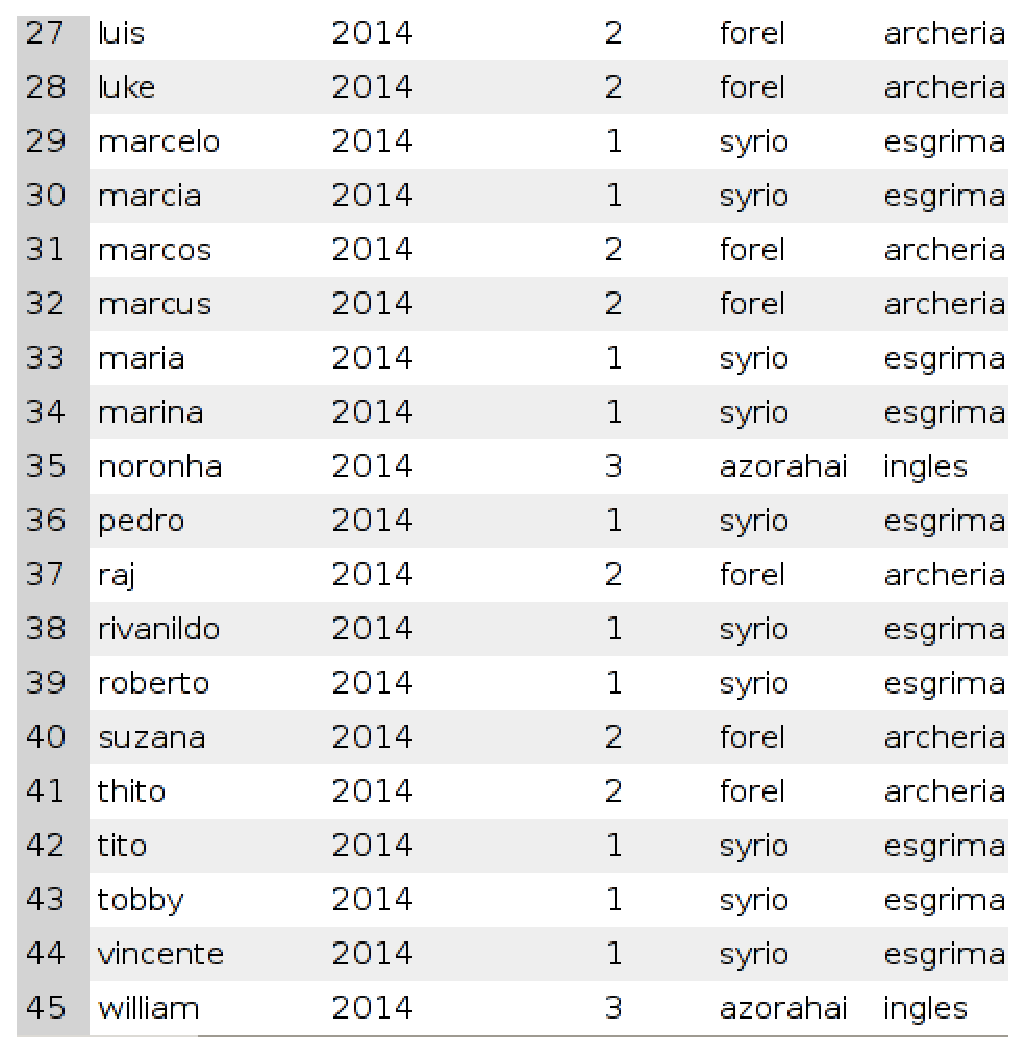
\includegraphics[width=.7\textwidth]{Figures/r12}
    \caption{Sa�da da Consulta 1 \textbf{parte 2}}
    \label{fig:r12}
\end{figure}

\subsubsection{\textbf{Consulta 2 - Boletim de notas}}

\begin{figure}[!h]
    \centering
    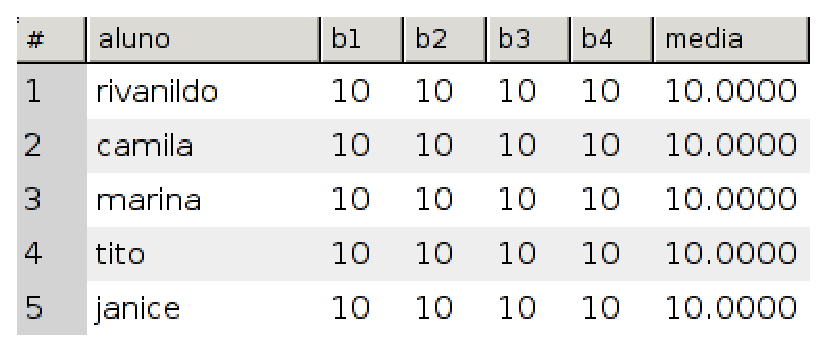
\includegraphics[width=.7\textwidth]{Figures/r2}
    \caption{Sa�da da Consulta 2}
    \label{fig:r2}
\end{figure}

\subsubsection{\textbf{Consulta 3 - Hist�rio cumulativo}}

\begin{figure}[!h]
    \centering
    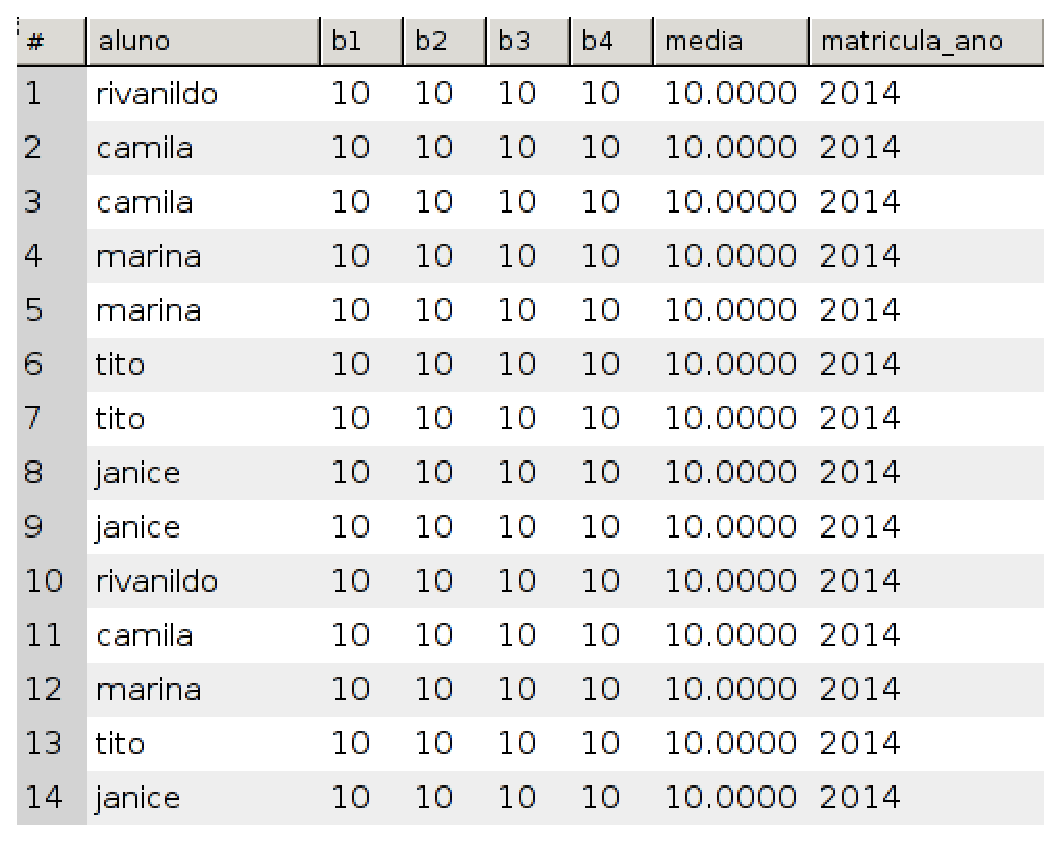
\includegraphics[width=.7\textwidth]{Figures/r3}
    \caption{Sa�da da Consulta 3}
    \label{fig:r3}
\end{figure}

\subsubsection{\textbf{Consulta 4 - Total de alunos em recupera��o por turma}}

\begin{figure}[!h]
    \centering
    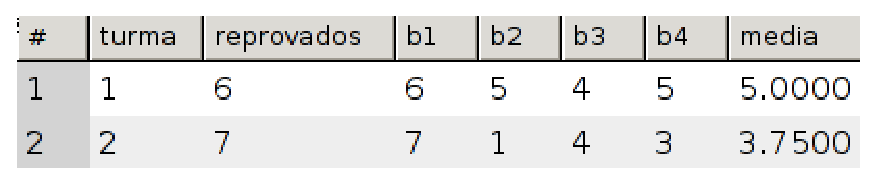
\includegraphics[width=.7\textwidth]{Figures/r4}
    \caption{Sa�da da Consulta 4}
    \label{fig:r4}
\end{figure}

\subsubsection{\textbf{Consulta 5 - Boleto Mensal (2 Respons�veis)}}

\begin{figure}[!h]
    \centering
    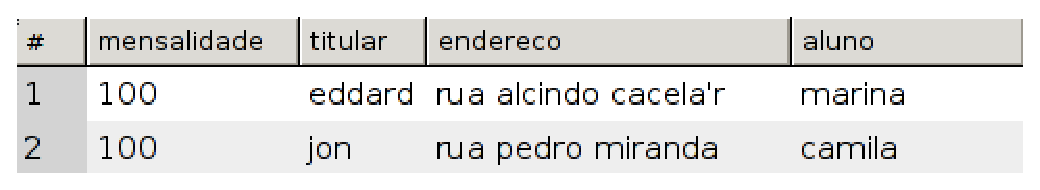
\includegraphics[width=.7\textwidth]{Figures/r5}
    \caption{Sa�da da Consulta 5}
    \label{fig:r5}
\end{figure}

\subsubsection{\textbf{Consulta 6 - Extrato do ano (3 alunos)}}

\begin{figure}[!h]
    \centering
    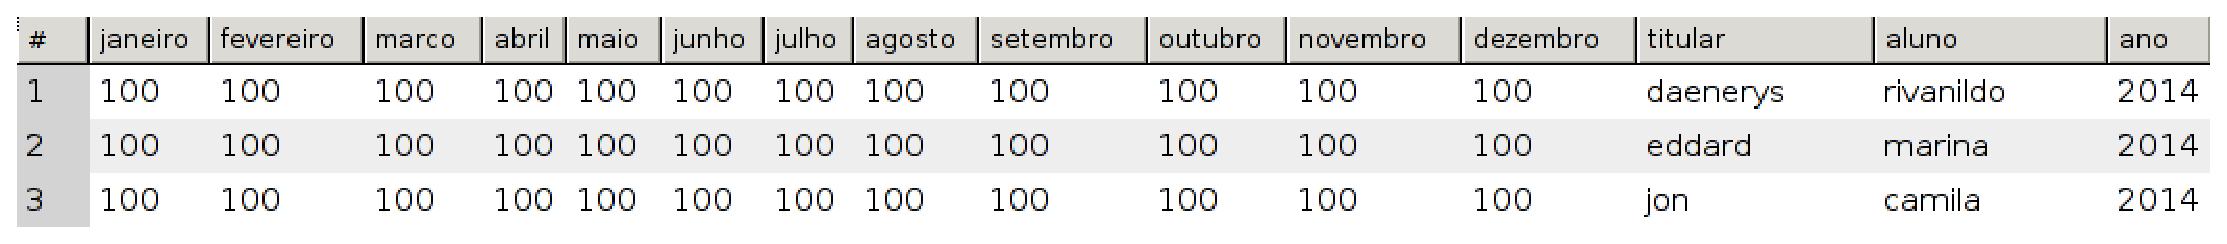
\includegraphics[width=.8\textwidth]{Figures/r6}
    \caption{Sa�da da Consulta 6 }
    \label{fig:r6}
\end{figure}


\end{section}
%%% EOF %%%
